\documentclass[outputdir=..]{sty/eiitfg}

% Hay muchos paquetes para LaTeX que facilitan centenares de trabajos
% engorrosos. Busca en Internet si no sabes hacer algo con LaTeX. El
% repositorio oficial está en https://ctan.org/

% Cambia los datos de tu TFG aquí
\title{Usa \LaTeX{} para elaborar tu TFG}
\author{Francisco Moya Fernández}
\email{francisco.moya@uclm.es}
\director{%
Francisco Moya Fernández\\
Fernando Castillo García}
\tfgid{XX-A/B-XXXXXX}
\gitrepo{https://github.com/FranciscoMoya/eii-tfg}

% Estos datos son opcionales. Si algún dato no quieres que figure borra la línea
\homepage{https://github.com/FranciscoMoya/eii-tfg}
\address{UCLM --- Escuela de Ingeniería Industrial\\
Campus Universitario de la Real Fábrica de Armas}
\zipcode{45071}
\phone{925 268 800 x.3729}


\begin{document}


% Puedes cambiar la licencia de este documento con la orden license.
%\license{Todos los derechos reservados.}

% Si usas muchos símbolos conviene que describas lo que significan en un archivo
% aparte (en este caso simbolos.tex).  Si no es el caso puedes comentar esta 
% línea
\listofsymbols{simbolos.tex}

\portada
\begin{agradecimientos}
Pon aquí tus agradecimientos, pero no te olvides de que se trata de un documento profesional.
\end{agradecimientos}	   
\begin{dedicatoria}
Aquí va la dedicatoria.
\end{dedicatoria}
\begin{resumen}
Aquí va el resumen en español. Entre 1000 y 1500 palabras (ver Anexo TFG-08). 

\warning{Escribe el resumen en estilo periodístico, desde lo más general a lo más específico.  Desde lo más importante a lo menos importante.  Esto último será especialmente útil cuando tengas que rellenar los \emph{Datos del TFG} en Campus Virtual.  En el formulario solo te permiten añadir un máximo de 600 palabras.  Si el resumen está en formato periodístico bastará con seleccionar los primeros párrafos.}
\end{resumen}

\begin{abstract}
Write here the abstract in english. It must be between 1000 and 1500 words long (see Anexo TFG-08).
\end{abstract}


\indices

% El cuerpo del documento está en la carpeta tex
% Aquí simplemente se incluyen los archivos correspondientes a cada capítulo.

% No los llames capitulo1, capitulo2, etc. Los números los pondrá LaTeX según
% el orden en que los pongas.  Eso facilitará después su posible reordenación
% o división.

% Esta estructura corresponde al anexo TFG-08b (documento científico-técnico).
% Si ves que tu proyecto concuerda con TFG-08a organiza el documento según
% UNE 157001

\chapter{Introducción} 
\label{ch:introduccion}

En este capítulo debes introducir el problema sin divagar, sin copiar de otros documentos y sin utilizar un lenguaje excesivamente técnico.  Tampoco utilices un lenguaje informal.  Este capítulo debería convencer al cliente de que el proyecto merece la pena.  Es decir, es un problema real y no está resuelto completamente.

Redacta la introducción al final del TFG, cuando tengas elaborado el capítulo de antecedentes, los resultados y su discusión.  De esta forma podrás evitar repetir argumentos que ya están en esos capítulos.  La introducción debe introducir también el contexto en el que se desarrolla el TFG.

Utiliza secciones y subsecciones para organizar el contenido del capítulo.  Utiliza preferentemente frases cortas.

Por cierto, el cliente es el que paga.  En el TFG el que paga es el tribunal y tu director o directores, en forma de calificación.  Así que a quien tienes que convencer es a ellos.  El tribunal no lo conocerás a priori.  Por eso la memoria debe estar escrita para que la entienda alguien que no es especialista en el campo de aplicación.  Pero eso no implica que se toleren la falta de rigor o la falta de argumentación técnica.  Solo implica que los argumentos específicos hay que explicarlos o citar la fuente que los explica.


\section{Organización de la memoria} 
\label{sec:organizacion-memoria}

La organización de este documento es conforme al anexo TFG-08b~\cite{tfg08b} de la Normativa Trabajo Fin de Grado de la Escuela de Ingeniería Industrial de Toledo, de la Universidad de Castilla-La Mancha, aprobada en Junta de Escuela el 23 de junio de 2016. Se descompone en los siguientes capítulos.

\begin{description}
    \item[Capítulo~\ref{ch:antecedentes}] Analiza los antecedentes y estado del arte en relación al tema del proyecto.
    \item[Capítulo~\ref{ch:objetivos}] Enumera y justifica los objetivos del proyecto y establece los límites intrínsecos y extrínsecos de ejecución del TFG.
    \item[Capítulo~\ref{ch:contribuciones}] Enumera las principales contribuciones y aportaciones personales del autor en este TFG.
    \item[Capítulo~\ref{ch:procedimiento}] Describe la metodología de desarrollo empleada durante la ejecución del TFG.
    \item[Capítulo~\ref{ch:resultados}] Describe en detalle las pruebas realizadas y los resultados obtenidos.
    \item[Capítulo~\ref{ch:discusion-resultados}] Discute los resultados en relación a los objetivos del proyecto.
    \item[Capítulo~\ref{ch:conclusiones}] Recopila las principales conclusiones del proyecto.
    \item[Anexos] Complementan la información del cuerpo del documento con información técnica útil para reproducir los resultados, pero innecesaria para comprender en su totalidad el TFG realizado.
\end{description}

\warning{Al finalizar el resto de los capítulos revisa esta descripción del documento para que coincida con lo que realmente contiene la memoria.  Por ejemplo, es frecuente fusionar varios capítulos en uno cuando son muy pequeños.  También es frecuente lo contrario, dividir un capítulo en varios cuando es muy extenso.}

\section{Repositorio de información}
\label{sec:repositorio}

Todo el material generado durante la ejecución de este proyecto está disponible en el repositorio \thegitrepo{}.  El material incluye el código \LaTeX{} del presente documento, el código fuente de los programas realizados o modificados, y todos los datos generados en la evaluación de resultados.
\chapter{Motivación y antecedentes}
\label{ch:antecedentes}

El problema que pretendes resolver está dentro de un contexto que el cliente debe conocer.  Esta sección aporta información para conocer en detalle la importancia del problema y la dificultad para resolverlo con los productos y programas disponibles actualmente.

Este capítulo concentrará el grueso de las citas del TFG.  Dado que se trata del primer trabajo profesional, el alumno no suele estar familiarizado con las citas bibliográficas.  Pon toda tu atención en qué citas y cómo lo citas.  Revisa la sección~\ref{sec:bibliografia-citas} para las reglas mínimas que deben cumplir las citas.

\warning{Es muy importante respetar la regla de atribuir correctamente.  No es aceptable desde el punto de vista legal, ni tampoco desde el punto de vista ético, copiar trabajo de otros sin atribuirlo correctamente a los autores.}

Esta sección debe estudiar de forma sistemática todas las opciones ya disponibles en la actualidad para resolver el problema. No basta con una mera enumeración, hay que estudiarlos mínimamente para explicar por qué no son una solución para el problema o qué podría aportar a la solución del problema.

Un método sistemático para realizar esta parte del TFG es la revisión sistemática de literatura, conocida habitualmente por sus siglas en inglés SLR (\emph{Sistematic Literature Review}).  Un resumen muy sencillo de cómo realizar una SLR puede encontrarse en~\cite{anderskofodpetersen2014}.  También encontrarás consejos prácticos en~\cite{sandroschulze2017}.  Para un proceso más detallado, especialmente si tu problema tiene mucho arte previo, puedes consultar~\cite{barbarakitchenhamstuartcharters2007}.  Si no hay mucho arte previo pon este capítulo y el siguiente juntos.

En una tesis doctoral el análisis sistemático del estado del arte es esencial. En un TFG es importante, pero no hay que perder la cabeza.  Un TFG son unas 300 horas de trabajo de un estudiante medio que ya posea los conocimientos generales necesarios (volveremos a esto más tarde).  Considero que un buen análisis del estado del arte corresponde a un trabajo de entre 25 horas y 100 horas, dependiendo del tema del proyecto.  Si el tema es muy específico es más fácil hacer el estudio del estado del arte.

Termina este capítulo con una sección que resuma el estado del arte e identifique las lagunas lo más claramente posible.  Una tabla comparativa o un gráfico pueden ser formas interesantes de presentar la información.
\chapter{Objetivos}
\label{ch:objetivos}

Primero enumera los objetivos, no los resumas ni los redactes en un párrafo.  Cada uno de los objetivos de un proyecto debe ser SMART:

\begin{description}
\item[Simple] Cada objetivo tiene que ser independiente, tener sentido por sí mismo y más o menos indivisible.  Si no es suficientemente indivisible, pero tiene sentido como una entidad independiente, debes descomponerlo en subobjetivos.
\item[Medible] Tiene que ser posible medir el grado de consecución al final del TFG.
\item[Acordado] Los objetivos no los pones tú solo.  Deben partir de un acuerdo con tu director.
\item[Realista] No pongas objetivos muy ambiciosos. Basta con que resuelva el problema de la forma más simple posible.  Si superas los objetivos nadie se va a quejar.  El director se encargará de que tampoco sean demasiado poco ambiciosos.
\item[Temporizado] Un objetivo debe tener un marco temporal. Si no es así el objetivo podría no cumplirse nunca.  Es difícil poner límites temporales muy estrictos en un primer proyecto de ingeniería, pero al menos acota.
\end{description}

Tras cada objetivo puedes añadir párrafos ampliando la descripción del objetivo, describiendo los límites y justificándolos.  También puedes describir de qué se parte.  Si es posible debería quedar plenamente justificado que se trata de objetivos SMART.  Considera tanto límites intrínsecos (inherentes a la definición del proyecto) como extrínsecos (limitaciones presupuestarias, equipamiento disponible, etc).
\chapter{Contribuciones}
\label{ch:contribuciones}

Tus contribuciones no tienen por qué limitarse al trabajo sistemático del TFG.  Puede que hayas contribuido en aspectos metodológicos, en ideas novedosas, en la planificación de experimentos, en desarrollos matemáticos.

Este capítulo está para agrupar todo eso.  Describe con claridad, y sin suponer conocimiento previo del desarrollo del proyecto (que viene después) todo lo que ha supuesto contribuciones originales por tu parte.
\chapter{Procedimiento}
\label{ch:procedimiento}

\info{Esta descripción está hecha a título orientativo. Puedes mejorarla con capturas de tu propio tablero Trello o con cualquier aclaración que consideres necesaria. Si andas corto de tiempo déjala como está.}

En el desarrollo de este TFG se ha utilizado una metodología ágil basada en \emph{Scrum}~\cite{scrumguide}, definida por el director.  El trabajo se ha dividido en iteraciones de dos semanas denominadas \emph{sprints}.  Las unidades de trabajo se presentan en forma de historias de usuario (\emph{user stories}) que definen mini-proyectos de muy corta duración que aportan valor al proyecto.  Es decir, cada historia de usuario cumple o ayuda a cumplir alguno de los objetivos.  Medir el valor percibido corresponde al propietario del producto (\emph{Product Owner}), que participa activamente en la planificación del proceso priorizando las unidades de trabajo.

La utilización de una metodología ágil permite equilibrar la cantidad de trabajo y los objetivos alcanzados.  Los 12 créditos ECTS del TFG se reparten según el criterio del director para que los resultados aporten el máximo valor posible, incluso en presencia de imprevistos.

\section{Diferencias con Scrum}

\emph{Scrum} es una metodología estrictamente centrada en el cliente.  El cliente es el responsable de priorizar y, en cierto modo, planificar las iteraciones.  Esto garantiza que la ejecución del proyecto responde al máximo con las expectativas del cliente, aún cuando los imprevistos impidan alcanzar alguno de los objetivos iniciales.  Esta característica de \emph{Scrum} es la única que se ha intentado mantener inalterada.  Sin embargo, el TFG es un proyecto individual, lo que ha requerido modificar significativamente otros aspectos de la metodología.

\subsection{Roles}

La única remuneración que se obtiene con la ejecución de un TFG es la calificación de los distintos aspectos (anteproyecto, valoración del director, valoración del tribunal, etc.).  Por tanto, el cliente del TFG se compone por el director y el tribunal de la defensa.  Desgraciadamente no es posible conocer a priori el tribunal.  Por este motivo el director es el único representante del cliente en el proceso de desarrollo (\emph{Product Owner}).

El TFG debe ser realizado de manera individual.  Por tanto, el equipo de trabajo (\emph{Team Member}) se compone exclusivamente por el autor.

La labor de dirección del TFG se asimila a la de dirección del proyecto y, por tanto, el director también actúa como coordinador del proceso, o \emph{Scrum Master}.  Nótese que hay dos roles representados por la misma persona.  Desde un punto de vista purista esto implica que puede haber conflicto de intereses y los intereses del cliente pueden estar insuficientemente representados.  Es una limitación extrínseca, que no es posible solucionar con el proceso actual.  Aún así, el uso de una metodología ágil centrada en el cliente debe mejorar el alineamiento de intereses cuando sobrevienen problemas que afectan o pueden afectar a la consecución de alguno de los objetivos iniciales.

\subsection{Historias de usuario}

\emph{Scrum}, como la mayoría de los métodos ágiles, está enfocada al desarrollo de proyectos en entornos de alta incertidumbre por equipos multidisciplinares bien formados.  El desarrollo de un TFG, al tratarse de un primer proyecto profesional, también está sometido a gran cantidad de incertidumbre.  Sin embargo, no siempre se cuenta con la formación previa necesaria para abordar todos los problemas.  Esto implica que, en ocasiones, se necesita aprender o leer, sin repercusión medible en el valor percibido por el \emph{Product Owner}.  En esos casos se planifican unidades de trabajo que no corresponden estrictamente a historias de usuario en el sentido de Scrum.  Se ha intentado mantener al mínimo este tipo de historias de usuario para tener el proceso lo más controlado posible.

Puntualmente ha sido necesario planificar historias de usuario que solo pretenden explorar opciones.  Este tipo de historias de usuario están contempladas en \emph{Scrum}, se denominan \emph{spikes}.  Sin embargo, en la ejecución de este TFG se ha procurado reducir al mínimo para que la exploración de alternativas no domine en el tiempo dedicado al TFG.

\subsection{Planificación de sprints}

Para la planificación y el seguimiento se ha utilizado un tablero \href{http://trello.com}{Trello}.  Los tableros Trello permiten agrupar tarjetas en una serie de listas con nombre.  Se ha utilizado el esquema propuesto en~\cite{andrewlittlefield2016}.

El autor ha sido responsable de añadir la mayoría de las historias de usuario a la lista \emph{Backlog}.  Se trata de un proceso continuo, durante toda la ejecución del proyecto.  El director, como \emph{product owner}, prioriza las historias, moviendo las tarjetas dentro de la lista \emph{Backlog}.  Justo antes de cada iteración se realiza una reunión presencial o virtual para revisar la iteración pasada y planificar la siguiente iteración.

Usando la técnica de \emph{planning poker} (ver~\cite{scrumguide}) se dimensionan las historias de usuario en días de trabajo.  Esta técnica consiste en un proceso de generación de consenso entre el autor y el director sobre el tiempo requerido para la ejecución de cada historia de usuario.  La unidad empleada ha sido de un día.

El director, como \emph{product owner} traslada las tarjetas correspondientes a las primeras historias de la lista \emph{Backlog} a la lista \emph{ToDo} hasta completar los 10 días de trabajo de la iteración.

\subsection{Flujo de trabajo}

El flujo de trabajo diario del autor corresponde a la siguiente secuencia:

\begin{itemize}
    \item Dentro de la lista \emph{ToDo} puede elegirse cualquier tarjeta para trabajar en ella.  Antes de comenzar el trabajo se arrastra la tarjeta a la lista \emph{Doing}.  Esto proporciona información en tiempo real al director del progreso de la iteración.
    
    \item Al terminar una historia de usuario la tarjeta correspondiente se arrastra a la lista \emph{QC} (quality control).
    
    \item El director, como \emph{Scrum Master}, revisa que la historia está realmente acabada y, si así es, la traslada a la lista \emph{Done}. En caso contrario la traslada a la lista \emph{Doing} otra vez, añadiendo un comentario que lo justifica.

    \item Si en el transcurso del trabajo se encuentra un obstáculo que impide progresar con una historia, se traslada a la lista \emph{Blocked}, añadiendo un comentario que lo justifica.
\end{itemize}

En todo momento es posible ver el estado global de ejecución del proyecto.  Al finalizar, la lista \emph{Done} contiene todas las historias de usuario ejecutadas por orden de terminación.  Y las listas \emph{Blocked} y \emph{Backlog} contienen (en este orden) todas las historias de usuario que corresponderían a trabajo futuro, ya priorizadas por el director.

\subsection{Herramientas de ayuda}

El proceso de desarrollo está fuertemente ligado a la herramienta \href{https://trello.com/}{Trello}.  Se trata de una herramienta colaborativa en línea, que permite mantener una serie de tarjetas agrupadas en listas con nombre.  Cada tarjeta puede tener un título, una descripción, un conjunto de adjuntos, y un conjunto de comentarios.  Trello se ha usado con éxito en la planificación de proyectos de nivel de complejidad muy variable.  Por ejemplo, Epic Games utiliza un tablero Trello para planificar las características a incorporar a cada nueva versión de Unreal Engine.  Por otro lado, un problema de Trello es el manejo limitado de la historia de modificaciones en las tarjetas y en los movimientos entre listas de tarjetas.  Esto dificulta en cierto modo el seguimiento de los cambios y, sobre todo, la corrección de errores en el proceso.  Por este motivo, Trello solo se ha empleado en la coordinación del trabajo, mientras que toda la gestión de cambios se ha delegado en otra herramienta.

Todo el proyecto ha sido gestionado desde su inicio con una herramienta de control de versiones distribuido~\cite{scottchaconbenstraub2018} en un repositorio público de GitHub, disponible en \thegitrepo.  Cada vez que se completa con éxito una historia de usuario se notifica mediante un comentario en la tarjeta correspondiente.  Este comentario tan solo contiene el identificador del paquete de cambios (\emph{commit}) que da por concluida la historia.  Todos los \emph{stakeholders} pueden consultar la evolución del proyecto en todo momento desde la propia página del repositorio.

 \warning{Es posible detallar en este capítulo las iteraciones desarrolladas.  Otra posibilidad es comentar brevemente los problemas encontrados y en el siguiente capítulo explicar los resultados globales.}

\chapter{Resultados}
\label{ch:resultados}

En el presente capítulo se recopila todos los resultados obtenidos a lo largo de este proyecto. Se encuentra divido en dos partes, una primera parte analítica y una segunda parte donde se desarrolla la proupesta inicial.
\begin{enumerate}
\item \textbf{Análisis de Universall®:} recoge los analisis téncnicos, funcionales y socioeconómicos de Universall®.
\item \textbf{Propuesta:} en esta parte se desarrolla la propuesta de actualización y renovación de la Escuela de Ingeniería de Toledo.
\end{enumerate}



\section{Analisis del ecosistema Universall®}

A continuación se detallan los análisis técnico, funcional y socioeconómicos que se han llevado a cabo en el dispositivo que vamos a emplar para desarrollar la propuesta.

Cabe destacar que el ecosistema Universall® está compuesto por hardware, software y casos de uso.

\subsection{Analisis Técnico de Universall}

En este capítulo se va a llevar  a cabo un analisis técnico del ecosistema Universall, el cual está compuesto tanto por una parte software como una hardware. La datos e información mostradas en este capítulo definen a Universall en términos generales, variando la composición de las partes en función de su aplicación final. Para nuestra apliación concreta se destinará un capítulo exclusivo definiendo el dispositivo que empleramos.

\begin{enumerate}
\item \textbf{HARDWARE}
\end{enumerate}

Universall es un dispositivo IoT que está compuesto por dos partes claramente diferenciadas: los quarks y omega.

\textbf{QUARKS}
Esta parte es la encargada de recopilar toda la información de cada uno de los sensores que componen el quark para más tarde enviarla a la nube para su análisis. En los quarks diferenciamos las siguientes caracterísitcas:
\begin{itemize}
\item Bluetooh 5.0: necesario para la comunicación entre los quarks y omega y entre los propios quarks.
\item Sensor 9D: hace referencia al conjunto de acelerómetro, giroscopio y brújula.
\begin{itemize}
\item Acelerómetro: mide aceleraciones y vibraciones, lo que hace posible saber si el dispositivo se está moviendo.
\item Giroscopio: mide la velicidad angular y detecta cuando el dispositivo está girando. 
\item Brújula: gracias a ella conoceremos la orientación en la que se encuentra nuestro dispositivo.
\end{itemize}
\item Sensor efecto Hall: es un sensor encargado de medir campos mágneticos y cuya función reside
\item Led multicolor: es programable en función del uso final que se dará al dispositivo. Gracias a su gama de colores pueden indicarse diferentes aspectos como si el dipositivo presenta batería baja, se está emparejando con los quarks o por ejemplo si está encendido.
\item Botón de presión: también es programable en función del uso final del producto y puede ser usado para mandar una alarma cuando se pulsa, para emparejarlos o para encenderlos.
\item Batería: puede ser de dos tipos:
\begin{itemize}
\item Pila: opción con una batería de botón intercambiable de 1000mAh cuya vida varía entre los 24 y 36 meses.
\item Batería recargable: opción que cuenta con una batería recargable de 80mAh con una vida aproximada de 3 años, que puede variar en función del uso del quark. 
\end{itemize}
\item Las dimensiones del quark son muy reducidas (30 x 30 x 10 mm).
\end{itemize}

\textbf{OMEGA}
Está parte es la encargada de recoger la información recopilada por los quraks y enviarla a la nube para que el usuario sea capaz de gestionar y analizar la información recogida. Omega está formado por:

\begin{itemize}
\item Wifi y/o NB-IoT: son las encargadas de enviar la información recogida a la nube a los servidores. El uso de una u otra dependerá de la aplicación final que tiene Universall.
\item Bluetooh 5.0:  necesario para la comunicación entre los quarks y omega
\item Batería no recargable: se trata de una batería de SoCl2 destinada a sistemas con una larga esperanza de vida. La estimación de vida de esta batería dependerá del número de conexiones que se realicen y de la cantidad de información subida, aunque se estima en 5 años.
\item USB-C: destinado a la conexión de omega con la red para no agotar la batería no recargable. 
\item Led multicolor: es programable en función del uso final que se dará al dispositivo. Gracias a su gama de colores pueden indicarse diferentes aspectos como si el dipositivo presenta batería baja, se está emparejando con los quarks o por ejemplo si está encendido.
\item Botón de presión: también es programable en función del uso final del producto y puede ser usado para mandar una alarma cuando se pulsa, para emparejarlos o para encenderlos.
\item Sensor efecto Hall: es un sensor encargado de 
\item Elementos opcionales:
\begin{itemize}
\item Sensor 9D
\item Sensor de temperatura
\item Sensor de humedad
\item Sensor de posición
\item Sensor de luz
\item Sensor de calidad del aire
\end{itemize}
\item Tiene unas dimensiones muy reducidas (115mm x 78mm x 35mm) 
\end{itemize}

\textbf{SOFTWARE}




\subsection{Analisis Socioeconómico de Universall}

En el presente capítulo se trata de abordar el funcionamiento del ecosistema completo de Universall, desde la recogida de información por parte de los sensores hasta su posterior análisis mediante Big Data.

\textbf{ELEMENTOS QUE INTERVIENEN}
En primer lugar definimos la función de cada uno de los componentes de Universall:
\begin{itemize}
\item Quark: es el conjunto de sensores que capta la información del entorno
\item Omega: es la base de comunicación que recoge la información de los quarks y la transmite a los servidores para posteriormente proceder a su análisis.
\end{itemize}

\textbf{FUNCIONAMIENTO}
El funcionamiento de Universall se divide en varias etapas que describimos a continuación que se pueden ver en la FIGURA

\begin{itemize}
\item Recopilación de información:
\end{itemize}

\begin{itemize}
\item Conexión con Omega:
\end{itemize}

\begin{itemize}
\item Subida de información a los servidores:
\end{itemize}

\begin{itemize}
\item Análisis de los datos:
\end{itemize}



\textbf{RIESGOS}




\subsection{Analisis Socioeconómico de Universall}

En este apartado se va a llevar  a cabo un analisis socioeconómico del ecosistema  Universall.

\textbf{ORIGEN}

Universall surge como una solución genérica para satiacer las necesidades de las empresas que quieran actulizarse para comenzar a estar conectados. Satisfacer dichas necesidades de una manera exclusiva en función del cliente provocaba el encarecimiento del producto destinado al cliente, así como su tiempo de entrega. Es este el factor clave del nacimiento de Universall, ya que es capaz de de gestionar las necesidades más demandadas y comunes, lo que hace que el tiempo de entrega sea mucho menor y su precio se vea claramente reducido pues el dispositivo es el mismo para cualquier cliente. 

\textbf{NECESIDADES}

Las necesidades que pueda llegar a satisfacer este producto van a estar siempre relacionadas con las exigencias del cliente y la apliación final que el mismo cliente busque. Es decir, no solo dependerá del hardware, sino tambien del sowtfare y del análisis que se realice de los datos recogidos. 

\textbf{APLICACIONES}

Como hemos comentado anteriormente, las aplicaciones siempre dependerán de las exigencias del cliente. Geeks!me ha desarrollado un cojunto de soluciones y casos de uso que incluyen tanto el hardware como el software para explotar el potencial de Universall, las cuales son:

\begin{itemize}
\item Universall Space™: destinada a hacer los espacios inteligentes y optimizar su uso. Con el se podría conocer datos como el tiempo medio de los descansos de un empleado o si una sala de reuiniones está libre o no en tiempo real.
\item Universall Care™: su objetivo principal es el cuidado de las personas mayores. Con el se podría hacer un seguimiento a distancia de la rutina que está llevando la persona, saber si ha salido de casa o si por ejemplo ha abierto el armario de las medicinas.
\item Universall Retail™: enfocado a los pequeños y grandes comercios con el que se podrán conocer el número de personas que entran al establecimiento o si por ejemplo la puerta está abierta o cerrada.
\item Universal Stars™: su función reside en el análisis del sueños de una persona. Esta apliación mostrará la actividad del sueño que esa persona ha tenido, y con la que se podrá conocer cómo descansa e incluso podrá aprender a dormir mejor.
\item Universal Safe™: esta aplicación está destinada a conocer el estado de nuestras propiedades en tiempo real, desde puertas y ventanas de la vivienda hasta un trastero.
\end{itemize}


\textbf{PRECIO}

El precio también varía en función de las necesidades del cliente. En términos generales se pueden establecer un rango de precios:
\begin{itemize}
\item Quarks: 25-30 €
\item Omega: 70-80€
\end{itemize}

\textbf{¿A QUIÉN VA DEDICADO?}

Universall busca satisfacer las demadas que puedan tener tanto una empresa como un particular, por lo que su modelo de negocio se puede resumir en dos vertientes: 

\begin{itemize}
\item B2B (Business to Business):
\item B2C (Business to Consumer):
\end{itemize}



\textbf{DAFO DE UNIVERSALL}

\begin{enumerate}
\item DEBILIDADES
\begin{itemize}

\item Es genérico. No está fabricado para un único cliente.
\item Cumple necesidades genéricas preestablecidas. No puede satisfacer otras necesidades fuera de ese rango.
\item Hardware y Software de código cerrado
\end{itemize}


\item FORTALEZAS

\begin{itemize}
\item Universal, cualquiera puede usarlo.
\item Satisface unas necesidades preestablecidas que pueden satisfacer un 80 de la demanda de peticiones.
\item Software y Hardware provisto por la empresa.
\item El uso del Big Data hace que su rango de aplicaciones sea grande.
\end{itemize}


\item OPORTUNIDADES

\begin{itemize}
\item Mercado del IoT aún por explotar.
\item Empresa joven y dinámica.
\end{itemize}


\item AMENAZAS
\begin{itemize}
\item Posibles competidores con productos similares:
\begin{itemize}
\item WhatsBee de BMates.
\item Family Safe de Intener of Things & Innovation.
\end{itemize}


\item Redes de comunicación aún en desarrollo: NB-IoT y LTE/M.
\item Altos costea de chips NB-IoT y LTE/M.
\item Temas relativos a la Privacidad y Seguridad
\end{itemize}
\end{enumerate}

\chapter{Discusión de resultados}
\label{ch:discusion-resultados}

La discusión de resultados se presenta de forma separada a los resultados propiamente dichos, porque de esta forma los resultados son directamente aprovechables en cualquier trabajo derivado.  Pero si el capítulo queda demasiado pequeño no dudes en mezclarlo con el anterior en un único capítulo de \emph{Resultados y discusión} o con el siguiente en un capítulo de \emph{Discusión de resultados y conclusiones}.
\chapter{Conclusiones}
\label{ch:conclusiones}

Las conclusiones deben cerrar el documento, destacando los aspectos más importantes de la ejecución del TFG.  Debe analizar qué objetivos se han alcanzado y en qué grado, qué objetivos se han tenido que dejar fuera del proyecto y por qué, y qué líneas de trabajo futuro abre el TFG.  Para esta última parte es especialmente útil la lista \emph{Blocked} y la lista \emph{Backlog} de tu tablero Trello.

En total las conclusiones no deberían superar dos o tres hojas.  Si ves que se alarga demasiado, traslada material al capítulo de discusión de resultados.

Fíjate en que los objetivos abren el trabajo personal y las conclusiones lo cierran.  Procura mantener un orden que resalte esta relación.


% La bibliografía la puedes descomponer en varios archivos .bib
% Los archivos .bib se pueden escribir a mano con ayuda de un editor online
% (e.g. http://truben.no/latex/bibtex) o generar con Mendeley u otro
% gestor de bibliografía. Solo se incluyen las referencias que son citadas
% en el texto.
\bibliography{bib/main,bib/how,bib/ejemplos}

\appendix

% Los apéndices pueden ir en la misma carpeta que el cuerpo del documento 
% porque eso facilita la migración de partes de un capítulo a un anexo.
\chapter{Chuleta de \LaTeX{}}
\label{ch:latex}

\LaTeX{} es un formato textual para construir documentos complejos, cualquier tipo de documento complejo.  No es difícil, y de hecho está pensado para que personas sin formación en tipografía y composición puedan redactar documentos estéticamente impecables.  Pero necesita algo de tiempo para acostumbrarse a la filosofía.

Puedes acabar tu TFG simplemente imitando la redacción de este documento, pero seguro que puedes sacar más partido si aprendes algo de \LaTeX{}.  Hay muchas guías sencillas para empezar. Por ejemplo,~\cite{ernestoaranda2013} o~\cite{gastonsimone2002} son resúmenes suficientemente completos y sencillos.  En caso de que quieras ampliar tus conocimientos tendrás que empezar por el libro de Leslie Lamport~\cite{leslielamport1994}, el creador de \LaTeX{}.  Procura complementarlo con~\cite{latexcompanion2004} y, especialmente, navegar por el \href{https://ctan.org}{CTAN} (\emph{Comprehensive \TeX{} Archive Network}).  CTAN es un repositorio enorme de paquetes, que facilitan la edición de todo tipo de detalles.  Desde las cabeceras de página, hasta la creación de enlaces hipertexto o el manejo de colores.

En este anexo se incluye un pequeño recetario, extraído de la plantilla de Fernando Castillo, que puedes usar a modo de recordatorio rápido, pero procura utilizar una referencia más completa cuando empieces a editar el documento.

\warning{Este recetario no es un libro de \LaTeX{}, ni es para sentarse a leerlo, es para usarlo cuando lo necesites.  No te mostramos cómo se escribe en \LaTeX{} cada ejemplo, sino que directamente lo hacemos.  Cuando necesites hacer algo semejante, mira el código de este documento en \url{https://github.com/FranciscoMoya/eii-tfg}}

\section{Texto} 
\label{sec:texto}

\noindent En esta sección se muestran ejemplos de efectos de texto.

\begin{description}
\item[\texttt{textbf}] \textbf{Texto en negrita.}

\item[\texttt{textit}] \textit{Texto en cursiva.}

\item[\texttt{underline}] \underline{Texto subrayado.}

\item[\texttt{large}] {\large Texto grande}

\item[\texttt{Large}] {\Large Texto más grande}

\item[\texttt{LARGE}] {\LARGE Texto mucho más grande}

\item[\texttt{textsc}] \textsc{Texto en versalitas}

\item[\texttt{textsf}] \textsf{Texto en fuente sans-serif}

\item[\texttt{texttt}] \texttt{Texto en fuente mono-espaciada}
\end{description}

A veces resulta útil este tipo de texto para funciones de programación o código fuente. Por ejemplo:

\begin{verbatim}
    [x,y]=function(t,z) 
\end{verbatim}

\subsection{Listas numeradas y con viñetas} 

Listas numeradas. Se utilizan cuando la posición que ocupan los elementos es importante, para contar los elementos, o cuando se necesita añadir referencias a algunos de los elementos.

\begin{enumerate}
\item diodos
\item transistores
    \begin{enumerate}
    \item transistores pnp
    \item transistores npn
    \item operacionales
    \end{enumerate}
\item operacionales
\end{enumerate}

Listas con viñetas. Se utilizan cuando la posición concreta de los elementos no es importante:

\begin{itemize}
\item diodos
\item transistores
    \begin{itemize}
    \item transistores pnp
    \item transistores npn
    \item operacionales
    \end{itemize}
\item operacionales
\end{itemize}

\section{Figuras}
\label{sec:figuras}

En esta sección se muestran algunos ejemplos de figuras.  La fig.~\ref{fig:figurita-ejemplo} es un ejemplo de \emph{Encapsulated PostScript}.  Se trata de un formato vectorial, que no se degrada al escalarlo.  Este tipo de formatos son los ideales para usar con \LaTeX{}.  Utiliza siempre que puedas imágenes en formato EPS o PDF.

\begin{figure}[hbtp]
\centering
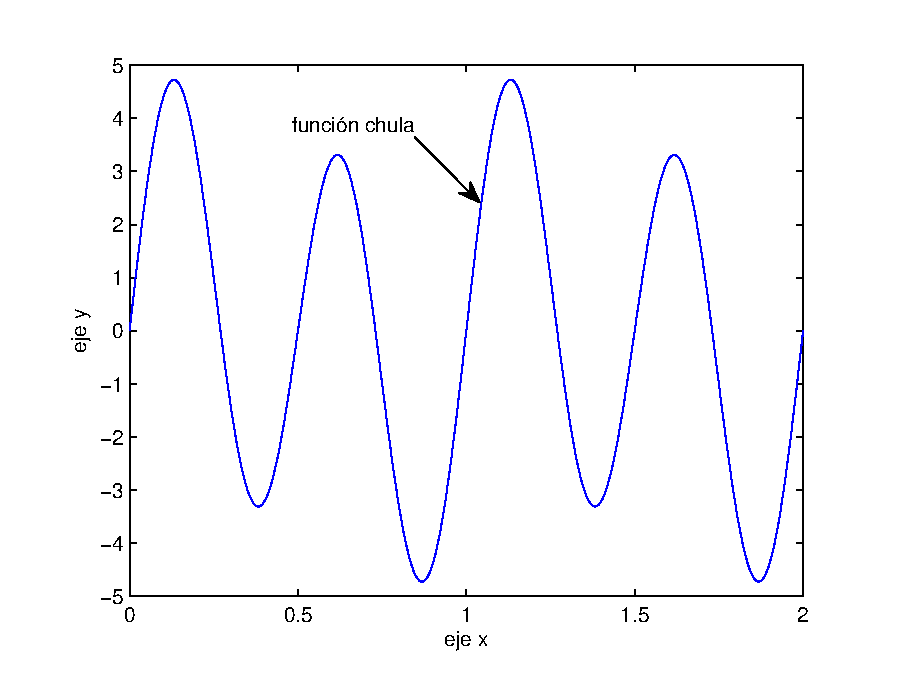
\includegraphics[scale=0.5]{ejemplo.eps}
\caption{Figurita ejemplo}
\label{fig:figurita-ejemplo}
\end{figure}

La forma de incluir la figura es simple:

\begin{lstlisting}[language={[LaTeX]TeX},frame=none,numbers=none]
\begin{figure}
\centering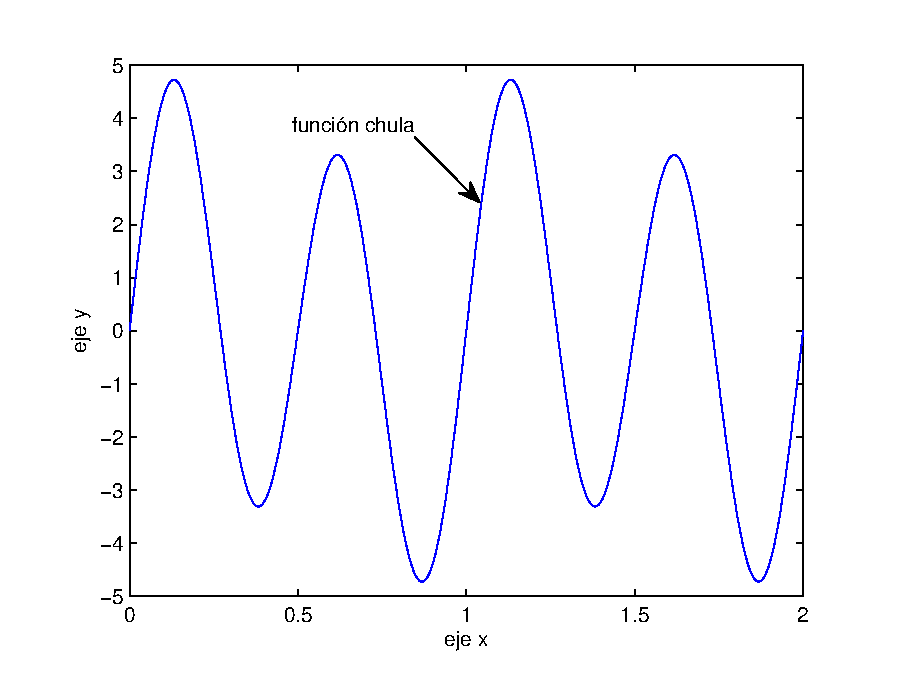
\includegraphics[width=6cm]{ejemplo.eps}
\caption{Figurita ejemplo}
\label{fig:figurita-ejemplo}
\end{figure}
\end{lstlisting}

El entorno \texttt{figure} crea un cuadro flotante, con todo el contenido de la figura, que \LaTeX{} coloca en el sitio menos malo.  La \texttt{caption} es el pie de la figura y la \texttt{label} es la etiqueta que nos permitirá referirnos a ella en el texto (con la orden \texttt{ref}).

\LaTeX{} utiliza un algoritmo nada evidente para colocar las figuras de manera que sea estéticamente agradable.  Pero tú puedes influir en las preferencias de colocación.  El entorno \texttt{figure} tiene un parámetro opcional entre corchetes que indica las opciones de colocación.  Por defecto es \texttt{[tbp]}, que equivale a \emph{top, bottom, page}.  Eso quiere decir que intenta primero ponerla a comienzo de página.  Si no lo consigue, al final de una página.  Y si así tampoco lo consigue, en una página entera, solo para la figura.  En este ejemplo utilizo las opciones \texttt{[hbtp]} para que intente la secuencia \emph{here, bottom, top, page}.  En este caso prefiero que la ponga debajo antes que arriba, para que no aparezca en una sección anterior.

Con \LaTeX{} puedes conseguir que las figuras no se muevan en absoluto, pero eso deja documentos extremadamente descompensados.  No lo hagas nunca.  Es mejor mover ligeramente la figura en el texto o incluso re-escribir parte del texto, antes de forzar la posición.  De todas formas, si no me quieres hacer caso, en la fig.~\ref{fig:figurita-ejemplo-2}  tienes un ejemplo que fuerza la posición.

\begin{figure}[h!]
\centering
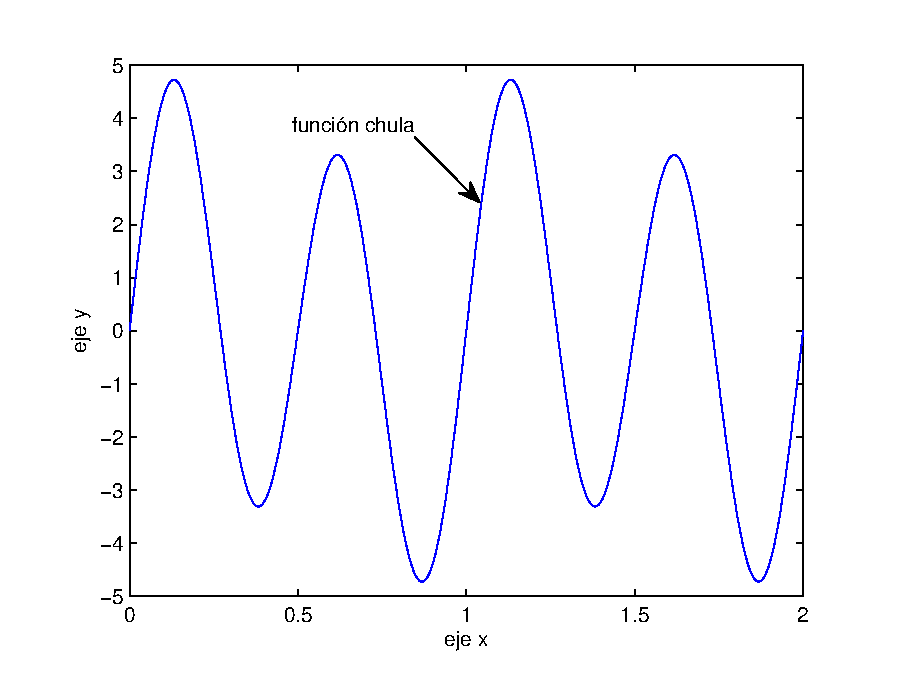
\includegraphics[scale=0.5, angle=15]{ejemplo.eps}
\caption{Figurita ejemplo 2}
\label{fig:figurita-ejemplo-2}
\end{figure}

Para poder poner figuras que no son de elaboración propia es necesario primero obtener permiso del autor y, además, añadir la fuente al pie de foto. Hay muchas guías de estilo que explican en detalle cómo hacerlo. Por ejemplo, la \emph{American Psychological Association} tiene un \href{https://www.lib.sfu.ca/help/research-assistance/format-type/online-images/citing#citing-images-in-apa}{capítulo específico de su manual de publicaciones}.  El manual de la APA se usa extensivamente en todo tipo de literatura científica.

\begin{figure}[htb]
\centering
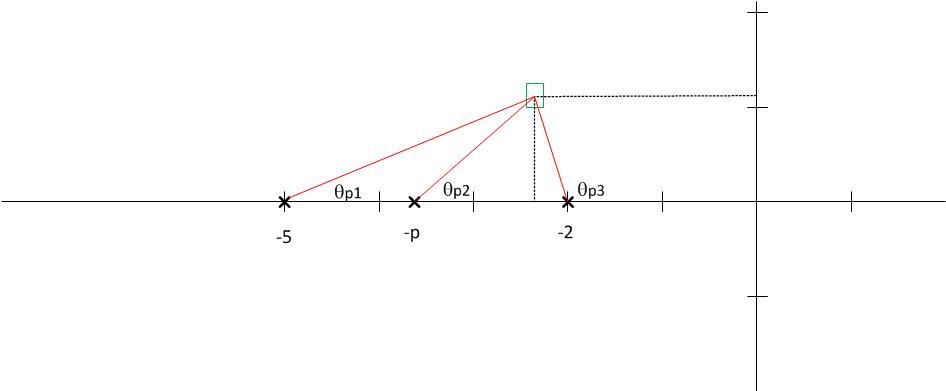
\includegraphics[scale = 0.5]{ejemplo2.jpg}
\caption{Figurita ejemplo 3. Extraída de la plantilla de TFG de Fernando Castillo. \copyright 2018 Fernando Castillo. Reproducida con permiso.}
\label{fig:figura-ejemplo-3}
\end{figure}

\warning{Fíjate bien.  No se citan las imágenes como si se tratara de referencias bibliográficas.  No debe haber pie de página (orden \texttt{footnote}) ni cita (orden \texttt{cite}) en un pie de foto (\texttt{caption}).  La atribución de la obra debe estar al mismo nivel que la obra usada.  Por eso debe atribuirse completamente en el pie de foto.  Si no te gusta como queda haz tus propias imágenes.}

Se puede controlar el escalado de la imagen y el ángulo de forma muy sencilla, con las opciones de la orden \texttt{includegraphics}.  En la fig.~\ref{fig:figura-ejemplo-3} se muestra un ejemplo de figura escalado a un 30\%.  La orden \texttt{includegraphics} ajusta los parámetros de la imagen para mantener la relación de aspecto original, si esto es posible.  Esto hace que podamos especificar simplemente el ancho o el alto deseado, que va a ser lo más habitual.  En mi opinión, las opciones más frecuentes de \texttt{includegraphics} son, por orden:

\begin{figure}
\centering
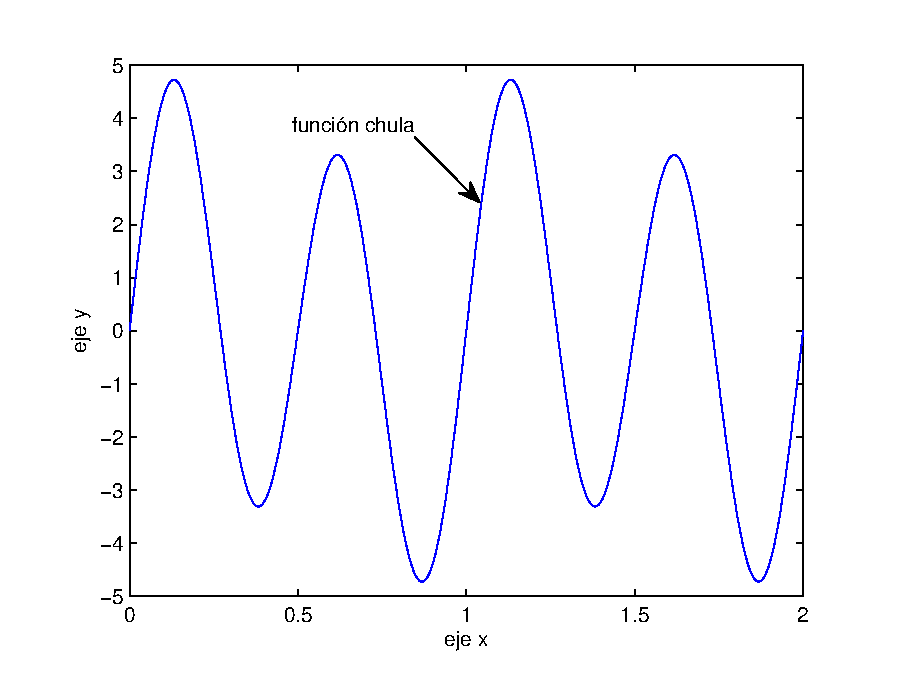
\includegraphics[width=\textwidth]{ejemplo.eps}
\caption{Figura ejemplo que ocupa todo el ancho del texto.}
\label{fig:figura-ejemplo-4}
\end{figure}

\begin{description}
\item[\texttt{width}]  Fija el ancho de la imagen.  Puede ser un tamaño absoluto en centímetros (\texttt{cm}), milímetros (\texttt{mm}) o puntos PostScript (\texttt{pt}).  Por ejemplo,  \verb|width=1.5cm|.  También puede ser un tamaño relativo a cualquier medida del documento.  Por ejemplo, \verb|width=0.5\textwidth| sería una figura que ocupe la mitad del ancho del texto.

\item[\texttt{height}] Fija la altura de la imagen.  Es similar a \texttt{width} pero con la altura.  Se puede especificar tanto altura como anchura, de manera que se modifica la relación de aspecto original.

\item[\texttt{scale}] Utiliza un factor de escala para la imagen.  Puede ser mayor de 1 para ampliar la imagen.

\item[\texttt{angle}] Gira la imagen un número de grados determinado.  Si el número es negativo el giro es en sentido horario.  Si es positivo el giro es antihorario.
\end{description}


En la fig.~\ref{fig:figura-angulo-30} se muestra un ejemplo de figura girada 30.

\begin{figure}[btp]
\centering
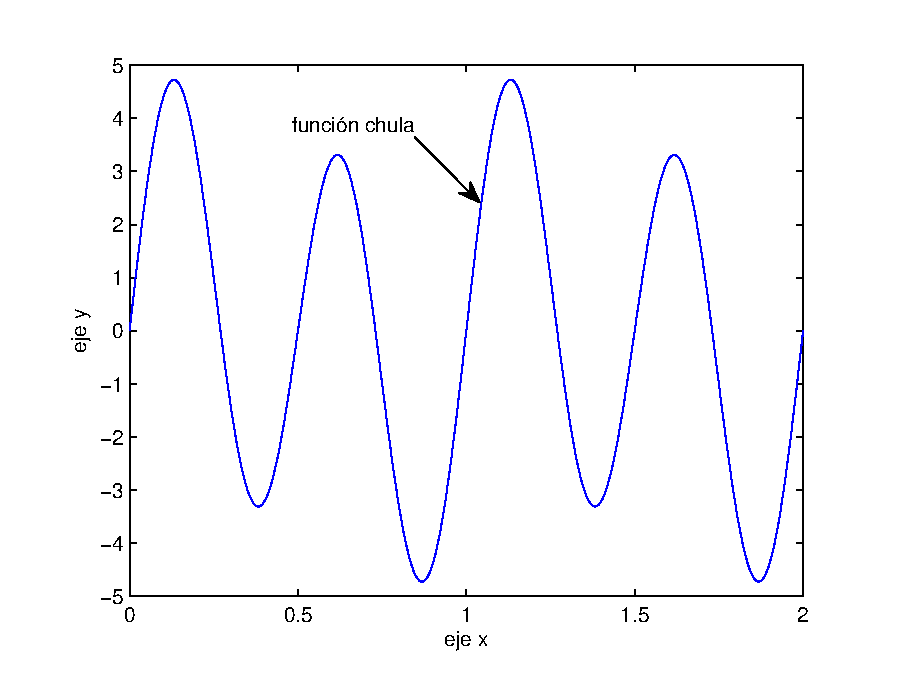
\includegraphics[width=.3\textwidth,angle=-30]{ejemplo.eps}
\caption{Figura ejemplo de rotación.}
\label{fig:figura-angulo-30}
\end{figure}

Una característica interesante del entorno \texttt{figure} es que permite definir sub-figuras con la orden \texttt{subfigure} o el entorno del mismo nombre.  La colocación de las sub-figuras es prácticamente automática.  Un ejemplo puede verse en la figura~\ref{fig:matriz-figuras}.

\begin{figure}[htbp]
\centering
\subfigure[figurita1]{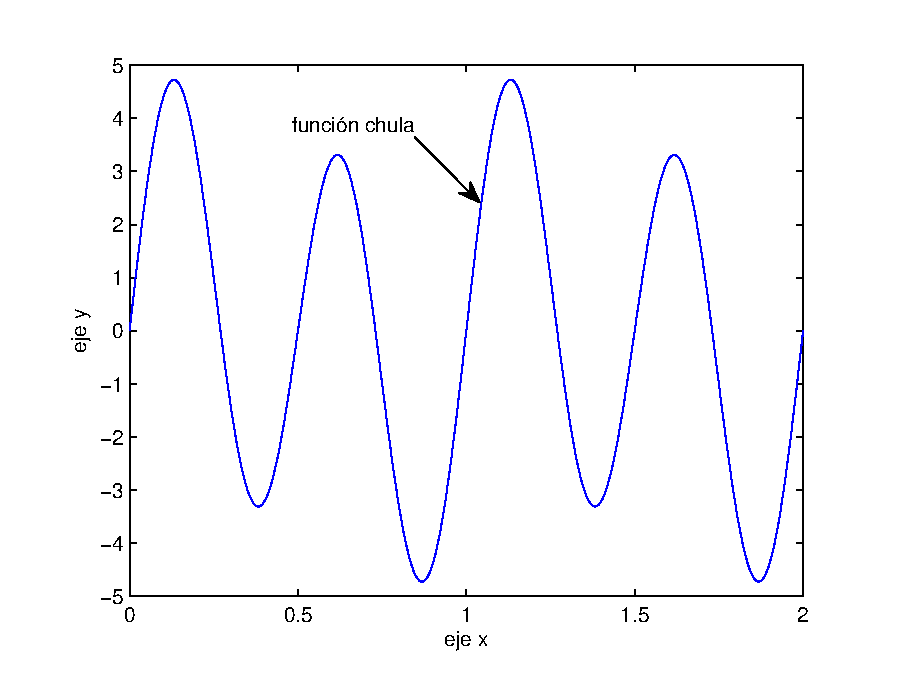
\includegraphics[width=40mm]{ejemplo.eps}}
\subfigure[figurita2]{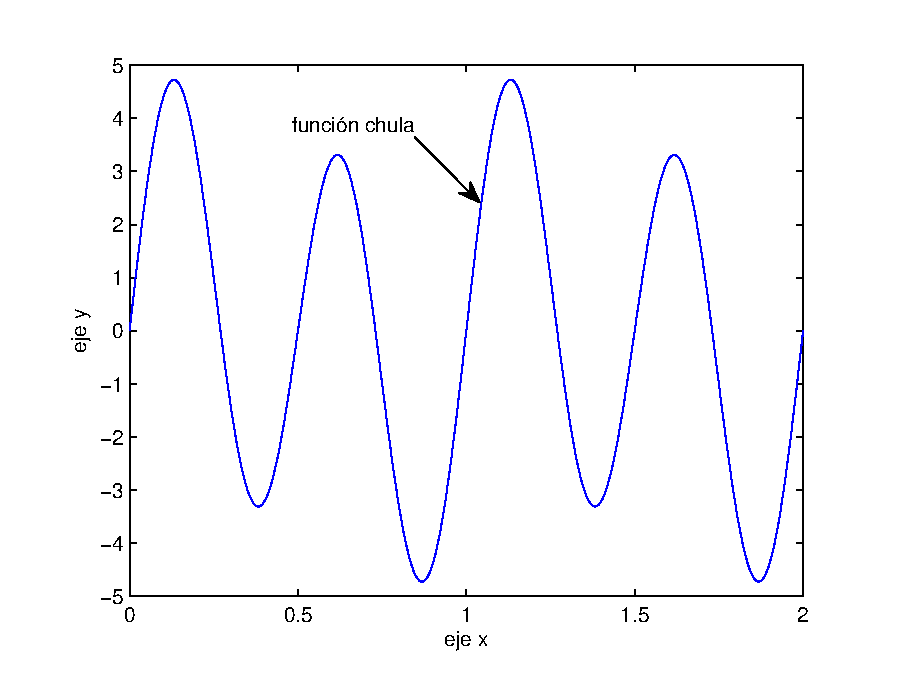
\includegraphics[width=40mm]{ejemplo.eps}}
\subfigure[figurita3]{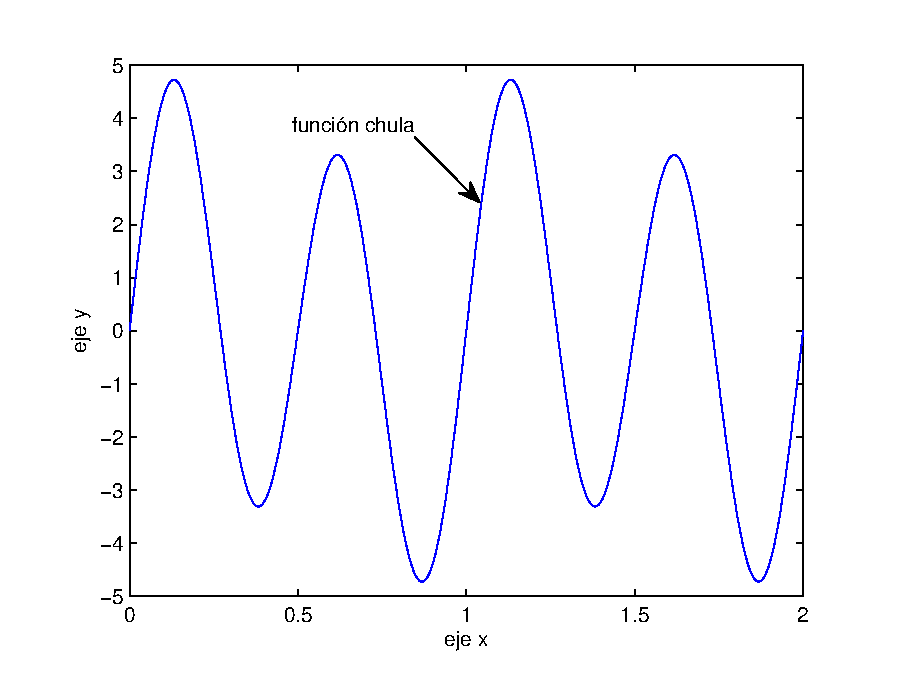
\includegraphics[width=80mm]{ejemplo.eps}}
\caption{Matriz de figuras} 
\label{fig:matriz-figuras}
\end{figure}

Una subfigura puede referenciarse a partir de la referencia a la figura.  Por ejemplo, la figura~\ref{fig:matriz-figuras}(a) es igual que la figura~\ref{fig:matriz-figuras}(b). Sin embargo, cuando las figuras son muy complejas, es posible que se prefieran esquemas más automáticos.  En \href{https://tex.stackexchange.com/questions/181225/how-to-reference-to-subfigure-in-latex}{StackExchange} encontrarás soluciones a éste y otros problemas con mucha facilidad.

En general, he tratado de mantener un compromiso entre el número de características incluidas y la facilidad de uso de la plantilla.  Las figuras muy complejas es algo que prefiero evitar, así que en el estilo de la plantilla no incorpora los paquetes \texttt{subcaption} y \texttt{cleveref}.

\section{Tablas} 
\label{sec:tablas}

En esta sección se muestran algunos ejemplos de tablas.

\begin{table}[htb]
\centering
\vspace{2mm}
\begin{tabular}{|c|c|c|}
\hline
 Regulador & Función de Transferencia & orden  \\
 \hline
 P         & $\alpha_1$               & 2      \\
 \hline
\end{tabular}
\caption{Resultados de la simulación}
\label{tab:resultados-simulacion}
\end{table}

Las tablas en \LaTeX{} no son complejas pero puedes simplificar aún más usando un editor interactivo de tablas.  Por ejemplo, en \url{https://truben.no/table/} hay una aplicación \emph{online} para editar multitud de formatos de tablas.  Es especialmente útil para tablas complicadas.

En \LaTeX{} es bastante frecuente separar la cabecera del cuerpo de la tabla poniendo dos \texttt{hline}, como en la tabla~\ref{tab:sencilla}.

\begin{table}[htb]
\begin{center}
\begin{tabular}{|l|l|}
\hline
País     &    Ciudad \\ \hline \hline
España   &    Madrid \\ \hline
España   &    Valencia \\ \hline
Francia  &    París \\ \hline
\end{tabular}
\caption{Tabla muy sencilla.}
\label{tab:sencilla}
\end{center}
\end{table}

La complejidad empieza cuando hay que expandir celdas para ocupar varias columnas o varias filas.  Por ejemplo, la tabla (\ref{tab:dificililla}) tiene una celda multi-columna y otra celda multi-fila.  En estos casos un editor interactivo como el de \href{https://truben.no/table/}{Peder Lång Skeidsvoll} puede ser de gran ayuda para un principiante.  Explora las opciones, no son evidentes al principio.

\begin{table}[htb] 
\centering
\begin{tabular}{|c|c|}
\hline
\multicolumn{2}{|c|}{Europa} \\
\hline
País  & Ciudad \\ \hline \hline
\multirow{2}{1.1cm}{España} & Madrid \\ \cline{2-2}
& Valencia \\ \hline
Francia & París \\ \hline
\end{tabular}
\caption{Fusionando celdas.}
\label{tab:dificililla}
\end{table}

Las tablas, al igual que las figuras, tienen un parámetro opcional entre corchetes que indican las preferencias de posición.  Se puede forzar pero, al igual que con las figuras, conduce a documentos muy descompensados.  Procura evitarlo.  Dentro de la tabla se define un entorno \texttt{tabular} que indica con su argumento obligatorio las columnas.  Este entorno es muy útil en cualquier organización matricial.  Se puede usar también para presentar las subfiguras de una figura, o para definir una matriz.

Las tablas muy largas deben dividirse en varias páginas.  En el estilo de este TFG hemos incluído el paquete \texttt{longtable}, que facilita enormemente escribir este tipo de tablas largas.  En ese caso, en lugar del entorno \texttt{table} y el entorno \texttt{tabular} se usaría solamente el entorno \texttt{longtable}, que es una especie de híbrido de los dos, con un montón de características opcionales.  Para ilustrar su uso reproducimos \href{https://texblog.org/2011/05/15/multi-page-tables-using-longtable/}{un ejemplo de TeXblog} en la tabla~\ref{tab:tabla-larga}.

\begin{center}
\begin{longtable}{|c|c|c|c|}
\caption{Un ejemplo de tabla larga}
\label{tab:tabla-larga}\\
\hline
\textbf{Primera} & \textbf{Segunda} & \textbf{Tercera} & \textbf{Cuarta} \\
\hline
\endfirsthead
\multicolumn{4}{c}%
{\scriptsize\textbf{\tablename\ \thetable}\ -- \textit{Continúa de la página anterior}} \\
\hline
\textbf{Primera} & \textbf{Segunda} & \textbf{Tercera} & \textbf{Cuarta} \\
\hline
\endhead
\hline \multicolumn{4}{r}{\textit{\scriptsize Continúa en la página siguiente}} \\
\endfoot
\hline
\endlastfoot
1 & 2 & 3 & 4 \\ 1 & 2 & 3 & 4 \\ 1 & 2 & 3 & 4 \\ 1 & 2 & 3 & 4 \\
1 & 2 & 3 & 4 \\ 1 & 2 & 3 & 4 \\ 1 & 2 & 3 & 4 \\ 1 & 2 & 3 & 4 \\
1 & 2 & 3 & 4 \\ 1 & 2 & 3 & 4 \\ 1 & 2 & 3 & 4 \\ 1 & 2 & 3 & 4 \\
1 & 2 & 3 & 4 \\ 1 & 2 & 3 & 4 \\ 1 & 2 & 3 & 4 \\ 1 & 2 & 3 & 4 \\
1 & 2 & 3 & 4 \\ 1 & 2 & 3 & 4 \\ 1 & 2 & 3 & 4 \\ 1 & 2 & 3 & 4 \\
1 & 2 & 3 & 4 \\ 1 & 2 & 3 & 4 \\ 1 & 2 & 3 & 4 \\ 1 & 2 & 3 & 4 \\
1 & 2 & 3 & 4 \\ 1 & 2 & 3 & 4 \\ 1 & 2 & 3 & 4 \\ 1 & 2 & 3 & 4 \\
1 & 2 & 3 & 4 \\ 1 & 2 & 3 & 4 \\ 1 & 2 & 3 & 4 \\ 1 & 2 & 3 & 4 \\
\end{longtable}
\end{center}
\section{Ecuaciones} 
\label{sec:ecuaciones}

Si hay algo donde \LaTeX{} es especialmente útil, es en las fórmulas matemáticas.  Prácticamente no hay otra opción cuando las fórmulas son relativamente complejas.  En esta sección se muestran algunos ejemplos de ecuaciones.

\begin{equation}
    \mathbf{v} = \left[
    \begin{array}{c}
        2 \\
        3 \\
        -4 
    \end{array}
    \right]
\end{equation}

En \LaTeX{} es trivial el uso de cualquier notación de vectores.  Tan solo hay que familiarizarse con las órdenes correspondientes.  Por ejemplo, en esta ecuación:

\begin{equation} 
\vec{F} = m \vec{a}
\label{eq:dinamica}
\end{equation}

donde $\vec{F}$ es la fuerza, $\vec{a}$ es la actitud y $m$ la masa.

Las ecuaciones pueden referenciarse igual que las figuras, las tablas o las secciones.  Por ejemplo, la ecuación~\ref{eq:dinamica2} \ldots

\begin{equation} 
\alpha_{inicial} = \beta^{final} + \gamma
\label{eq:dinamica2}
\end{equation}

\begin{equation}
G(s)=\frac{(s^2+s+1)^2}{s^3+1}
\label{eq:dinamica3}
\end{equation}

El uso de letras griegas o símbolos matemáticos es también muy sencillo.  Tan solo hay que familiarizarse con la orden que los inserta.  Puede parecer difícil, pero basta con ojear una chuleta como \href{https://www.colorado.edu/physics/phys4610/phys4610_sp15/PHYS4610_sp15/Home_files/LaTeXSymbols.pdf}{ésta}\footnote{\url{https://www.colorado.edu/physics/phys4610/phys4610_sp15/PHYS4610_sp15/Home_files/LaTeXSymbols.pdf}}.

La ecuación~\ref{eq:transformacion} muestra un ejemplo de integral.  También es muy sencillo, puesto que la notación de los límites coincide con la de los subíndices y superíndices.

\begin{equation}
F(y) =  \int_{x_a}^{x_b} K(x,y) f(x) dx
\label{eq:transformacion}
\end{equation}

Cuando se necesita un entorno tabular dentro de un entorno matemático se utiliza el entorno \texttt{array}. La ecuación~\ref{eq:matriz} muestra un ejemplo.

\begin{equation}
\left(
\begin{array}{cccc}
1 & 0 & \cdots & 0 \\
0 & 1 & \cdots & 0 \\
\vdots & \vdots & \ddots & \vdots \\
0 & 0 & \cdots & 1
\end{array}
\right)
\label{eq:matriz}
\end{equation}

\section{Bibliografía, citas y referencias} 
\label{sec:bibliografia-citas}

Otro de los aspectos especialmente cuidados de \LaTeX{} es el manejo de bibliografía y citas.  En esta plantilla utilizamos el paquete \emph{natbib}.  Es un paquete muy flexible que permite adaptarse a casi cualquier estilo de citas existente.  Sin embargo, en los documentos de ingeniería suele haber bastante consenso en el estilo que hemos configurado en la plantilla.  A menos que tengas un motivo, no lo cambies.

La bibliografía en \LaTeX{} se hace con ayuda de unos archivos auxiliares escritos en formato BibTeX.  Es otro formato textual, con una serie de campos que hay que rellenar.  Para la composición de entradas BibTeX lo más sencillo es utilizar un editor online, como \url{http://truben.no/latex/bibtex/}.  Ten presente que algunos tipos de entradas pueden no estar configurados en el estilo de bibliografía que usas.  Por ejemplo, \emph{Online} y \emph{URL}, que aparecen en el editor en línea, no están en el estilo de bibliografía que usamos en esta plantilla.  Usa en su lugar \emph{Misc} como en el archivo \texttt{bib/how.bib} de esta plantilla.  En principio todas las entradas de bibliografía que utilices en tu TFG deben ponerse en \texttt{bib/main.bib}.

Con \LaTeX{} estándar se cita empleando la orden \texttt{cite} con el campo clave que contiene todo registro de BibTeX.  Esto puede valer, pero en el paquete \texttt{natbib}, se recomienda emplear \texttt{citep} en su lugar.  Por ejemplo, según el trabajo~\citep{armas2011estimation} \ldots mientras que según~\citep{castillo2010design} el control es una cosa muy buena. 

Con \texttt{natbib} tienes otra opción de cita, con la orden \texttt{citet}, que también se usa, especialmente cuando se quiere destacar el autor.  Por ejemplo, según \citet{castillo2011time} la potencia sin control no sirve de nada.  Puedes usar cualquiera de los dos estilos de cita, pero debes ser consistente.  La inconsistencia confunde al lector.

Una referencia bibliográfica se utiliza como argumento de autoridad, para dar peso a tu propia argumentación.  Por tanto, hay tres elementos clave que siempre deben estar: 
\begin{itemize}
    \item El autor, puesto que palabras anónimas no dan peso a nada.  Recuerda que el autor es lo que da peso a tu argumento.  No cites artículos divulgativos, ni autores sin un mínimo prestigio en el campo de lo que afirman.
    \item El título, puesto que el lector debe poder buscar por sí mismo el documento original.
    \item La fecha, puesto que un mismo autor puede cambiar de opinión a lo largo de su vida.  Por ejemplo  John Maynard Keynes es Premio Nobel pero tiene numerosos escritos contradictorios.  Su opinión era bastante cambiante con el tiempo.
\end{itemize}

Si falta alguno de estos elementos no es una referencia y no se cita.  Se puede poner como una nota a pié de página (\texttt{footnote}) o como una URL en el cuerpo del texto, pero no como una referencia.

Por cierto, es conveniente citar las fuentes.  Es decir, debes tomarte la molestia de buscar quién dijo o inventó lo que citas y dónde lo publicó por primera vez.  Es la mínima cortesía que se debe tener con los colegas de profesión.  Supongo que tú también querrás crédito por tu trabajo en tu futuro profesional.
		
\section{Hojas de datos}
\label{sec:hojas-datos}

Esto es un ejemplo de anexo. En la figura~\ref{fig:hoja-datos} se muestra la hoja de especificaciones del motor empleado.

\begin{figure}[ht!]
\centering
\fbox{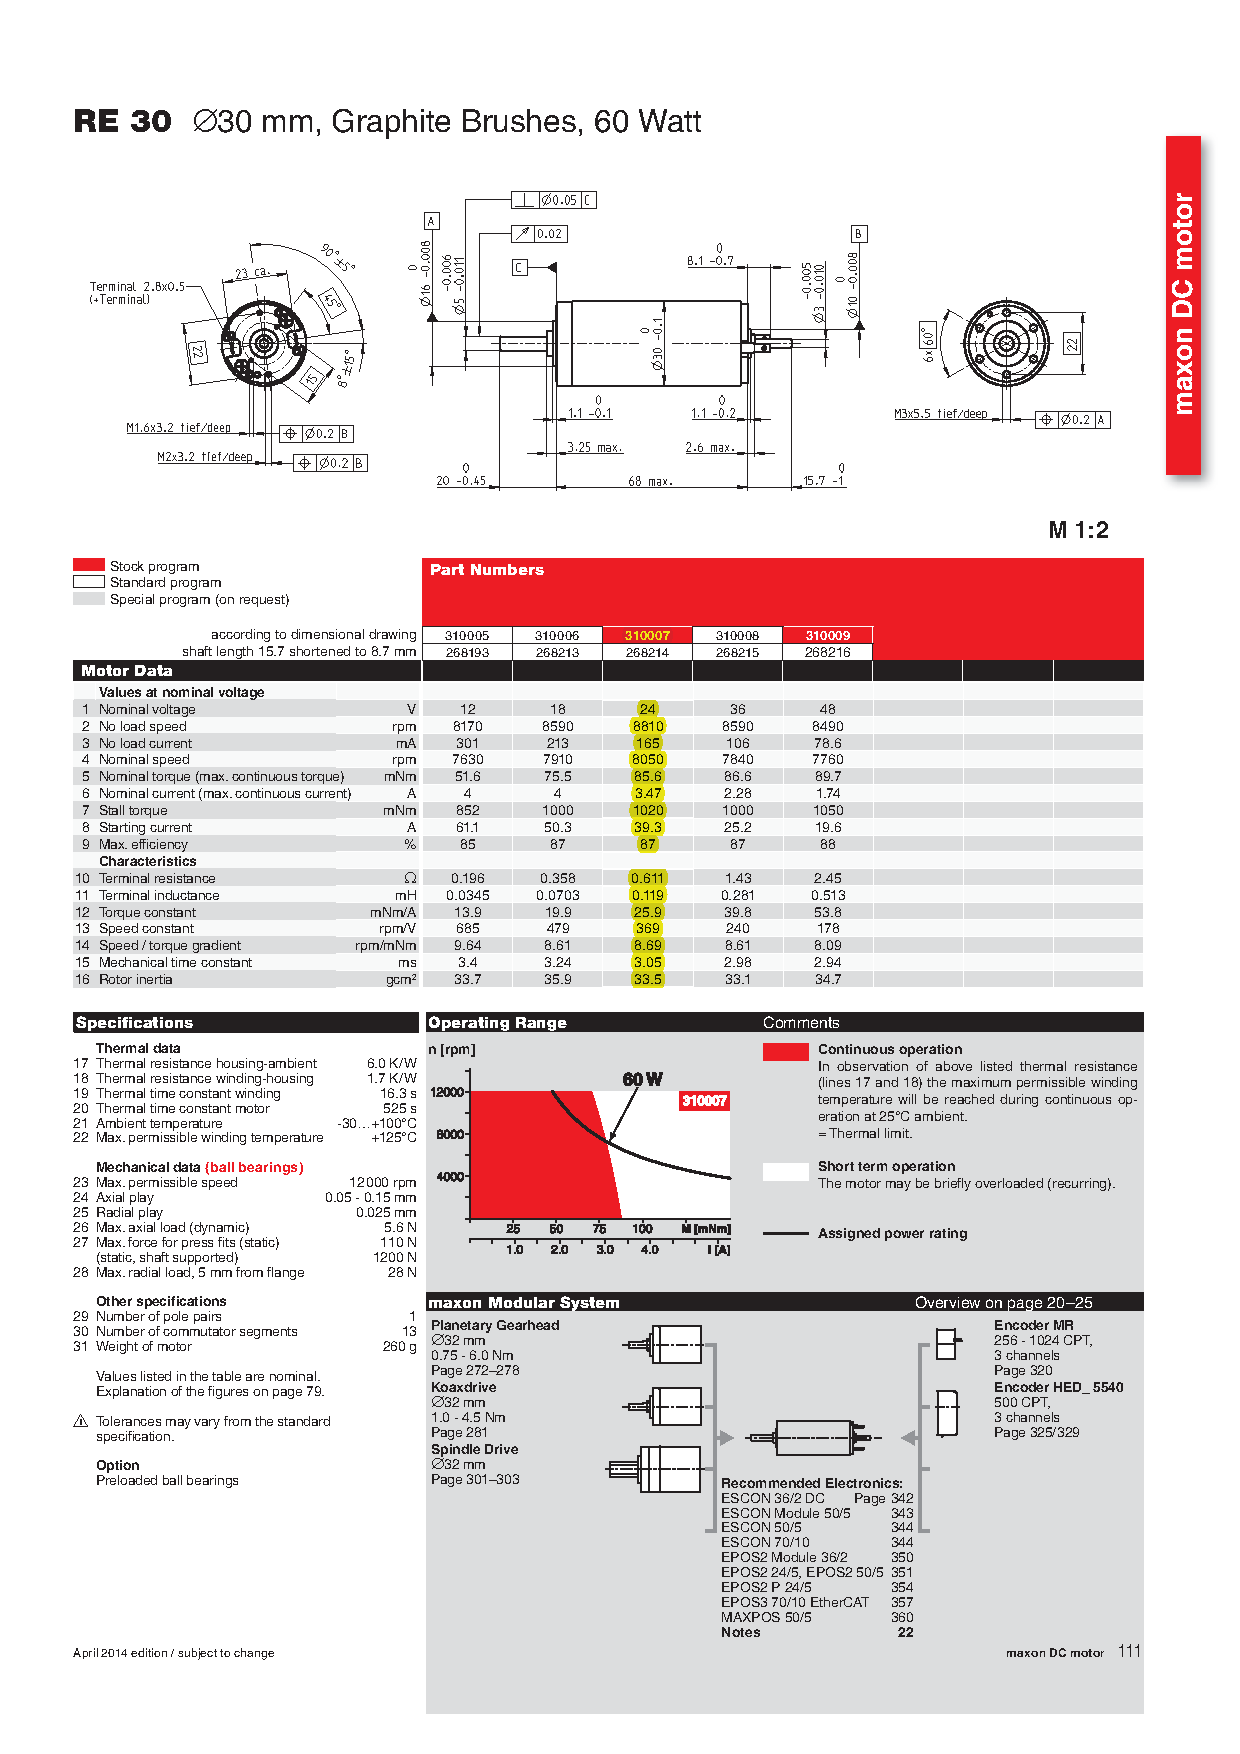
\includegraphics[width=.95\textwidth]{RE30.pdf}}
\caption{Figura ejemplo. Tomada de hoja de catálogo de \href{https://www.maxonmotor.com/medias/sys_master/root/8830469472286/2018EN-129.pdf}{motores DC con escobillas de grafito de Maxon} \copyright~2014 Maxon Motors. Reproducida con permiso.}
\label{fig:hoja-datos}
\end{figure}	
\section{Código fuente} 
\label{sec:codigo-fuente}

Esto es un ejemplo de anexo. En este anexo se muestran algunos ejemplos de como plasmar código fuente.

En mi opinión, la forma más flexible y cómoda es usar el paquete \texttt{lstlistings}.  Permite incluir archivos o parte de archivos directamente del proyecto con la orden \texttt{lstinputlisting}.

\lstinputlisting[language=Matlab,
    caption={Ejercicio 20 como texto incorporado},
    label=src:ej20-input
]{memoria/tex/latex/ejercicio20.m}

O bien se puede copiar el texto del programa o fragmento en un entorno \texttt{lstlisting} con las mismas opciones que la orden \texttt{lstinputlisting}.

\begin{lstlisting}[language=Matlab,
    caption={Ejercicio 20 como texto en línea.},
    label=src:ej20-online
]
function [T]=Ejercicio20(f,c)

T = char('B'*ones(8,8));

for i=1:8
    for j=1:8
        if ( (i==f) || (j==c) || (i+j==f+c) || (i-j==f-c) )
            T(i,j)='*';
        elseif ( rem(i+j,2)~=0 )
            T(i,j)='N';
        end
    end
end

T(f,c)='R';
\end{lstlisting}

\info{Te recomendamos que incluyas los archivos o parte de los archivos directamente del código de tu proyecto, ya sea mediante \texttt{lstinputlisting} o mediante \texttt{inputminted}.  De esta forma mantendrás sincronizado el documento con el código fuente.}

\noindent El paquete \texttt{lstlisting} te permite quitar los números y el marco, cuando el código se incluye como parte del texto. 

\begin{lstlisting}[language=Matlab,
    frame=none,numbers=none
]
function [T]=Ejercicio20(f,c)

T = char('B'*ones(8,8));

for i=1:8
    for j=1:8
        if ( (i==f) || (j==c) || (i+j==f+c) || (i-j==f-c) )
            T(i,j)='*';
        elseif ( rem(i+j,2)~=0 )
            T(i,j)='N';
        end
    end
end

T(f,c)='R';
\end{lstlisting}

\noindent Otra forma de incluir código es mediante el entorno \texttt{verbatim}.  Este método no tiene resalte de sintaxis ni facilidades de ningún tipo para definir etiquetas o numerar las líneas. 

\begin{verbatim}
function [T]=Ejercicio20(f,c)

T = char('B'*ones(8,8));

for i=1:8
  for j=1:8
    if ( (i==f) || (j==c) || (i+j==f+c) || (i-j==f-c) )
      T(i,j)='*';
    elseif ( rem(i+j,2)~=0 )
      T(i,j)='N';
    end
  end
end

T(f,c)='R';
\end{verbatim}

\noindent Otra forma alternativa a \texttt{lstlisting} es el paquete \texttt{minted}, que colorea el programa según el lenguaje empleado.  Puede resultar más agradable desde el punto de vista estético pero recuerda que las fotocopias en color son entre 5 y 10 veces más caras que las fotocopias en blanco y negro.

\begin{minted}{matlab}
function [T]=Ejercicio20(f,c)

T = char('B'*ones(8,8));

for i=1:8
    for j=1:8
        if ( (i==f) || (j==c) || (i+j==f+c) || (i-j==f-c) )
            T(i,j)='*';
        elseif ( rem(i+j,2)~=0 )
            T(i,j)='N';
        end
    end
end

T(f,c)='R';
\end{minted}




\end{document}
